%%%%%%%%%%%%%%%%%%%% author.tex %%%%%%%%%%%%%%%%%%%%%%%%%%%%%%%%%%%
%
% sample root file for your "contribution" to a proceedings volume
%
% Use this file as a template for your own input.
%
%%%%%%%%%%%%%%%% Springer %%%%%%%%%%%%%%%%%%%%%%%%%%%%%%%%%%


\documentclass{svproc}
%\documentclass[graybox]{svmult}
% RECOMMENDED %%%%%%%%%%%%%%%%%%%%%%%%%%%%%%%%%%%%%%%%%%%%%%%%%%%
%

% to typeset URLs, URIs, and DOIs
\usepackage{url}
\usepackage{hyperref}
\usepackage{helvet}         % selects Helvetica as sans-serif font
\usepackage{courier}        % selects Courier as typewriter font
%\usepackage{type1cm}        % activate if the above 3 fonts are
                           % not available on your system
\usepackage{color}
\usepackage{makeidx}         % allows index generation
\usepackage{graphicx}        % standard LaTeX graphics tool
\usepackage[misc]{ifsym}                            % when including figure files
\usepackage{multicol}        % used for the two-column index
\usepackage[bottom]{footmisc}% places footnotes at page bottom
\usepackage{tabularx}
\usepackage{multirow}
\usepackage{natbib}
\usepackage{algorithm}
\usepackage{algorithmic}
\usepackage[center]{caption}
\usepackage{longtable}
\usepackage{rotating}
 \usepackage{amsmath}
\usepackage{subfigure}
\usepackage[cp1251]{inputenc}
\def\UrlFont{\rmfamily}



\usepackage{graphicx}%
\usepackage{multirow}%
\usepackage{amsmath,amssymb,amsfonts}%
\usepackage{amsthm}%
\usepackage{mathrsfs}%
\usepackage[title]{appendix}%
\usepackage{xcolor}%
\usepackage{textcomp}%
\usepackage{manyfoot}%
\usepackage{booktabs}%
\usepackage{algorithm}%
\usepackage{algorithmicx}%
\usepackage{algpseudocode}%
\usepackage{listings}%
\usepackage{tikz}%
\usetikzlibrary{positioning,arrows.meta}%


%  Cột căn trái cho bảng
\usepackage{array}
\usepackage{ragged2e}
\newcolumntype{L}[1]{>{\RaggedRight\arraybackslash}p{#1}}


%comment
\usepackage{verbatim}

% References
\usepackage[numbers,sort&compress]{natbib}
\renewcommand{\bibname}{References}
\renewcommand{\bibsection}{\section*{\bibname}}



\begin{document}
\mainmatter              % start of a contribution
%
\title{A Multi-Agent LLM Architecture for Natural Language Access to Relational Business Data}
%
\titlerunning{NL2SQL Multi-Agent}  % abbreviated title (for running head)
%                                     also used for the TOC unless
%                                     \toctitle is used
%
\author{Tien Thanh Pham\inst{1} \and Tuan-Dat Trinh\inst{1}}
%
\authorrunning{Pham et al.  } % abbreviated author list (for running head)
%
%%%% list of authors for the TOC (use if author list has to be modified)
\tocauthor{Tien Thanh Pham, Tuan-Dat Trinh}
%
\institute{School of Information and Communications Technology, Hanoi, Vietnam\\
\email{tienthanhtk11@icloud.com, dattt@soict.hust.edu.vn}}

\maketitle              % typeset the title of the contribution

\begin{abstract}
Natural Language to SQL (NL2SQL) reduces the barrier between business users and relational data, yet large language model (LLM){-}based systems still struggle with schema grounding, join selection, aggregation, and nested logic.
This paper presents an application-oriented study of a six-stage multi-agent NL2SQL pipeline with explicit reasoning checkpoints: Question Analysis, Schema Selection, Query Planning, SQL Generation, SQL Refinement, and SQL Validation. Rather than treating SQL generation as a single step, the architecture isolates key decision points to improve error control.
The system is evaluated under a fixed protocol on the Spider 1.0 development split (1,034 questions), adopted due to the unavailability of the official test server. The proposed pipeline achieves 77.8\% Exact Match (EM) and 85.6\% Execution Accuracy (EX), outperforming a matched 4-stage baseline (73.7\% EM, 81.2\% EX).
\textcolor{red}{The system is evaluated under a fixed protocol on the Spider 1.0 development split (1,034 questions), adopted due to the unavailability of the official test server. The proposed pipeline achieves 73.6\% Exact Match (EM) and 84.9\% Execution Accuracy (EX), outperforming a matched 4-stage baseline (57.4\% EM, 84.9\% EX).}

These results indicate that explicit reasoning decomposition improves robustness, particularly for structurally complex queries. However, the gains cannot yet be cleanly attributed to the architecture itself, as they may partly stem from the increased inference budget.
The paper therefore frames the contribution as a controlled architectural study rather than a leaderboard claim, and reports detailed configuration settings to support reproducibility.

\keywords{NL2SQL, Text-to-SQL, multi-agent systems, large language models, business analytics, decision support}
\end{abstract}

\section{Introduction}
\label{sec:intro}

Natural Language to SQL (NL2SQL) translates natural language questions into executable SQL queries over relational databases, enabling non-technical users to access structured data without writing code. This capability is central to business analytics and decision-support systems.

Despite recent advances in large language models (LLMs), NL2SQL remains challenging for queries requiring multi-step reasoning. Typical failure modes include incorrect output fields, invalid join paths, missing aggregation constraints, and syntactically correct SQL queries that appear plausible but fail to reflect the actual intent of the question. 
%These errors are particularly pronounced on cross-domain Text-to-SQL benchmarks such as Spider, where training and evaluation are conducted on different databases, requiring systems to generalize across new schemas and query structures.

A common limitation of existing NL2SQL systems is their reliance on centralized generation. In such designs, schema grounding, join reasoning, aggregation, and output selection are implicitly entangled within a single generation step. As a result, early-stage reasoning errors are rarely recoverable and often propagate to the final query.

This paper investigates whether explicitly decomposing NL2SQL into intermediate reasoning stages improves robustness in complex query generation. We propose a six-stage pipeline consisting of (1) Question Analysis, (2) Schema Selection, (3) Query Planning, (4) SQL Generation, (5) SQL Refinement, and  (6) SQL Validation. Each stage focuses on a distinct reasoning task, producing explicit intermediate outputs that serve as inputs to subsequent stages. 

The system is evaluated on Spider 1.0~\cite{yu2018spider}, a widely used cross-domain Text-to-SQL benchmark in which training and evaluation use different database schemas to assess cross-schema generalization. Since official evaluation on the hidden Spider 1.0 test set requires submission to a dedicated evaluation server that is no longer operational, all experiments in this study are conducted on the development split.

The proposed 6-step pipeline achieves 77.8\% Exact Match (EM) and 85.6\% Execution Accuracy (EX), outperforming a matched 4-step baseline (73.7\% EM, 81.2\% EX). While these results suggest that explicit reasoning decomposition may improve SQL generation accuracy, the current study does not fully isolate the benefits of decomposition from the additional inference budget required by the multi-stage architecture.

\textcolor{red}{The proposed 6-step pipeline achieves 73.6\% Exact Match (EM) and 84.9\% Execution Accuracy (EX), outperforming a matched 4-step baseline (57.4\% EM, 84.9\% EX). While these results suggest that explicit reasoning decomposition may improve structural match to gold SQL, the current study does not fully isolate the benefits of decomposition from the additional inference budget required by the multi-stage architecture.}

All reported results are obtained with a single fixed configuration of models and hyperparameters (model assignment and parameters in Table~\ref{tab:repro}), selected through internal benchmarking before the final evaluation runs and kept unchanged across all experiments.


This work makes three main contributions. (i) First, it proposes an explicit reasoning-decomposition framework for NL2SQL in which intermediate decisions are externalized rather than remaining implicit, enabling inspection, refinement, and improved error containment throughout the generation process. (ii) Second, it provides a controlled empirical comparison between a reduced 4-stage baseline and the full 6-stage architecture on the Spider development split, enabling a systematic assessment of the impact of reasoning decomposition under a consistent experimental setup. (iii) Third, it presents a detailed analysis of performance across query difficulty levels and recurring error categories, offering insights into where multi-stage decomposition is most beneficial and where limitations remain.


% The contributions of this work are threefold. (i) First, we present a six-stage NL2SQL architecture that separates question understanding, schema grounding, planning, generation, refinement, and validation into explicit reasoning stages. (ii) Second, we perform a controlled architectural study on the Spider 1.0 development split by comparing the proposed pipeline with reduced variants under a consistent evaluation protocol. (iii) Third, we analyze performance across query difficulty levels and recurring error patterns to better understand the potential benefits and limitations of reasoning decomposition in NL2SQL systems.

% The main contributions are as follows:
% \begin{itemize}
%   \item A six-stage NL2SQL pipeline that explicitly separates analysis, schema grounding, planning, generation, refinement, and validation.
%   \item A controlled comparison between a reduced 4-step baseline and the full 6-step pipeline under the same evaluation protocol on the Spider development split.
%   \item An empirical analysis of performance across difficulty levels and recurring error patterns to identify where decomposition is most effective.
%   \item A contextual positioning against representative Spider-based systems to situate the proposed approach within existing decomposition and prompting paradigms.
% \end{itemize}

% \textbf{Venue positioning:} This work focuses on controlled architectural evaluation rather than leaderboard performance, providing reproducible evidence on the effect of explicit reasoning decomposition in NL2SQL systems.

\section{Related Work}
\label{sec:related}

Early neural Text-to-SQL systems, such as the feedback-driven neural semantic parser of Iyer et al.~\cite{iyer2017neural} and SyntaxSQLNet~\cite{yu2018syntaxsqlnet}, established the task of translating natural language questions into executable SQL queries. The introduction of Spider~\cite{yu2018spider} shifted the focus toward cross-domain generalization, requiring models to reason over previously unseen database schemas. Subsequent systems, including RAT-SQL~\cite{wang2020ratsql}, BRIDGE~\cite{lin2020bridge}, and RESDSQL~\cite{li2023resdsql}, substantially improved schema-aware representation and schema linking, leading to stronger performance on complex multi-table queries.


The emergence of large language models (LLMs) further transformed the NL2SQL landscape. Prompting-based approaches such as DIN-SQL~\cite{pourreza2023dinsql} and DAIL-SQL~\cite{gao2023dailsql} demonstrated that general-purpose LLMs can generate competitive SQL without task-specific decoders. Nevertheless, SQL generation is commonly performed within a single generation stage, making errors in schema grounding, join selection, or aggregation difficult to detect before they propagate to the final query.

To address these limitations, recent studies have increasingly explored explicit reasoning decomposition, iterative refinement, and multi-agent collaboration. SGU-SQL~\cite{zhang2025sgusql} introduces structure-aware decomposition to improve schema linking and SQL construction, while MAC-SQL~\cite{wang2025macsql} coordinates selector, decomposer, and refiner agents to improve execution accuracy through multi-agent collaboration. More general reasoning frameworks such as Reflexion~\cite{shinn2023reflexion}, CRITIC~\cite{gou2024critic}, AutoGen~\cite{wang2023autogen}, LangChain~\footnote{\url{https://www.langchain.com/}}, and CrewAI\footnote{\url{https://github.com/crewAIInc/crewAI}} further demonstrate the benefits of iterative reasoning and coordinated agents for complex language tasks. Building on this direction, DIVER~\cite{nan2026diver} integrates interactive tool use, dynamic value linking, and evidence-based reasoning to improve robustness in more realistic Text-to-SQL scenarios. Complementary approaches, including constrained decoding with PICARD~\cite{scholak2021picard}, improve syntactic validity through decoder-level constraints rather than reasoning decomposition.

Despite these advances, existing systems typically combine multiple design choices, including prompting strategies, model selection, tool use, refinement, and execution-guided repair, making it difficult to isolate the contribution of explicit reasoning decomposition itself. In contrast, this work investigates reasoning decomposition as the primary architectural variable through a controlled comparison between reduced and full multi-stage pipelines under a consistent experimental setting, providing empirical evidence on how explicit reasoning decomposition influences SQL generation accuracy and robustness.

% Despite these advances, existing systems frequently integrate multiple design choices, including prompting strategies, model selection, tool use, refinement, and execution-guided repair, making it difficult to isolate the contribution of explicit reasoning decomposition itself. In contrast, this work investigates explicit reasoning decomposition as the primary architectural variable through a controlled comparison between reduced and full multi-stage pipelines, providing empirical evidence for its impact on SQL generation performance under a consistent experimental setting.

% \section{Related work}
% \label{sec:related}

% Early Text-to-SQL systems such as Seq2SQL~\cite{iyer2017neural} and SyntaxSQLNet~\cite{yu2018syntaxsqlnet} established the task of translating questions into SQL. With Spider~\cite{yu2018spider}, research shifted toward cross-domain generalization, schema linking, and multi-table reasoning. Later systems such as RAT-SQL~\cite{wang2020ratsql}, BRIDGE~\cite{lin2020bridge}, and RESDSQL~\cite{li2023resdsql} improved schema-aware parsing, but most still relied on centralized generation.


% LLM-based approaches expanded the design space further. Prompting systems such as DIN-SQL~\cite{pourreza2023dinsql} and DAIL-SQL~\cite{gao2023dailsql} showed that strong language models can produce competitive SQL without specialized decoders, but they still struggle with output field choice, join selection, and aggregation logic. More recent decomposition-oriented systems push this direction further: SGU-SQL~\cite{zhang2025sgusql} combines structure-aware linking with syntax-guided subtask decomposition, while ReCAPAgent-SQL and its SSEV variant~\cite{wang2025macsql} combine planning, critique, self-refinement, and voting-style repair to improve execution performance.

% Another line of work focuses on explicit reasoning, self-correction, and multi-agent coordination. Reflexion~\cite{shinn2023reflexion} and CRITIC~\cite{gou2024critic} illustrate the value of critique stages, while AutoGen~\cite{wang2023autogen}, LangChain~\cite{chase2024langchain}, and CrewAI~\cite{moura2024crewai} support task decomposition through cooperating agents. Robustness-oriented systems such as DIVER~\cite{nan2026diver} further introduce dynamic value linking and evidence reasoning through interactive tool use, especially for harder real-world settings beyond standard benchmarks. We also note constrained decoding methods such as PICARD~\cite{scholak2021picard}, which improve output validity from a different angle than our decomposition strategy, and newer Spider-oriented systems such as SGU-SQL~\cite{zhang2025sgusql} and SSEV / ReCAPAgent-SQL~\cite{wang2025macsql}, which report strong dev-set results through structure-aware decomposition, refinement, and execution-guided repair. Our paper is closest in spirit to decomposition-based LLM NL2SQL systems, but it emphasizes explicit reasoning checkpoints and a matched internal comparison between reduced and full pipelines rather than a broad claim of benchmark leadership.

% Because prior studies often differ in backbone models, prompting strategies, and evaluation splits, numeric comparisons with prior work in this paper are contextual only, not apples-to-apples evidence.

\section{Proposed architecture}
\label{sec:arch}

\subsection{Architecture Overview}
\label{subsec:arch-overview}

The proposed framework decomposes the NL2SQL process into six sequential reasoning stages, each responsible for a distinct subproblem in the overall query generation workflow: (1) Question Analysis, (2) Schema Selection, (3) Query Planning, (4) SQL Generation, (5) SQL Refinement, (6) SQL Validation.


Each stage performs a dedicated reasoning function while passing its output to the next stage. Question Analysis identifies the user's intent and expected outputs. Schema Selection identifies the subset of tables and columns that are most relevant to the question, reducing irrelevant schema context before SQL generation. Query Planning constructs a high-level execution strategy before SQL is produced. SQL Generation translates the reasoning results into an executable SQL query. SQL Refinement performs semantic improvement on the generated query, and SQL Validation verifies syntactic correctness, schema consistency, and executability.


The overall architecture of the proposed six-stage reasoning pipeline is illustrated in Figure~\ref{fig:pipeline6}.
Table~\ref{tab:agents} details the inputs, outputs, and primary responsibilities of each reasoning stage.

To isolate the effect of explicit reasoning decomposition, we construct a reduced four-stage baseline that uses the same inputs and produces the same final output while removing the Query Planning and SQL Refinement stages. Instead, these reasoning responsibilities are absorbed into the SQL Generation stage. Figure~\ref{fig:pipeline4} illustrates the resulting baseline architecture.


\begin{figure}[t]
\centering
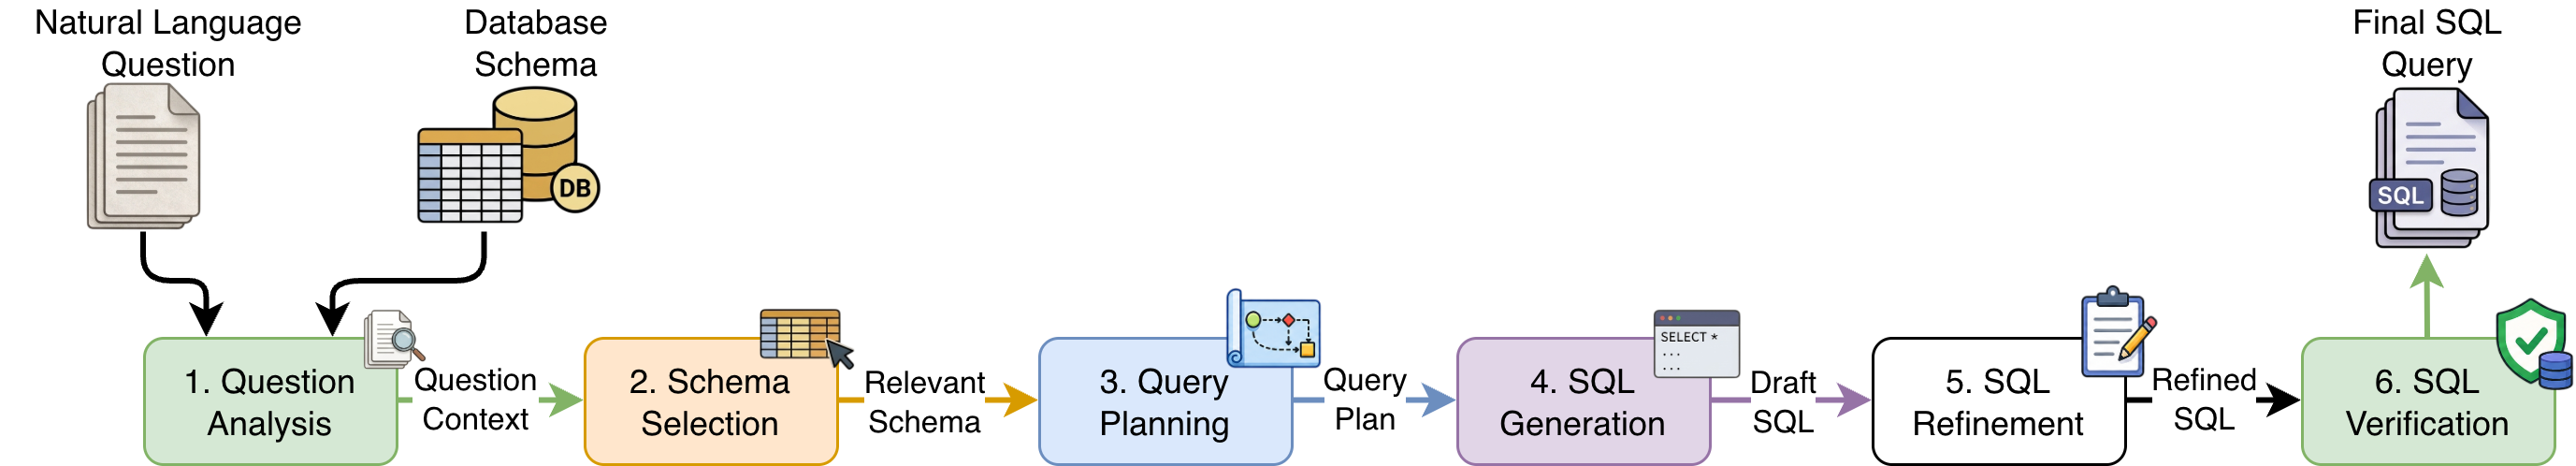
\includegraphics[width=\textwidth]{Figures/pipeline6.png}
\caption{Overview of the proposed six-stage NL2SQL reasoning architecture.}
\label{fig:pipeline6}
\end{figure}


\begin{figure}[t]
\centering
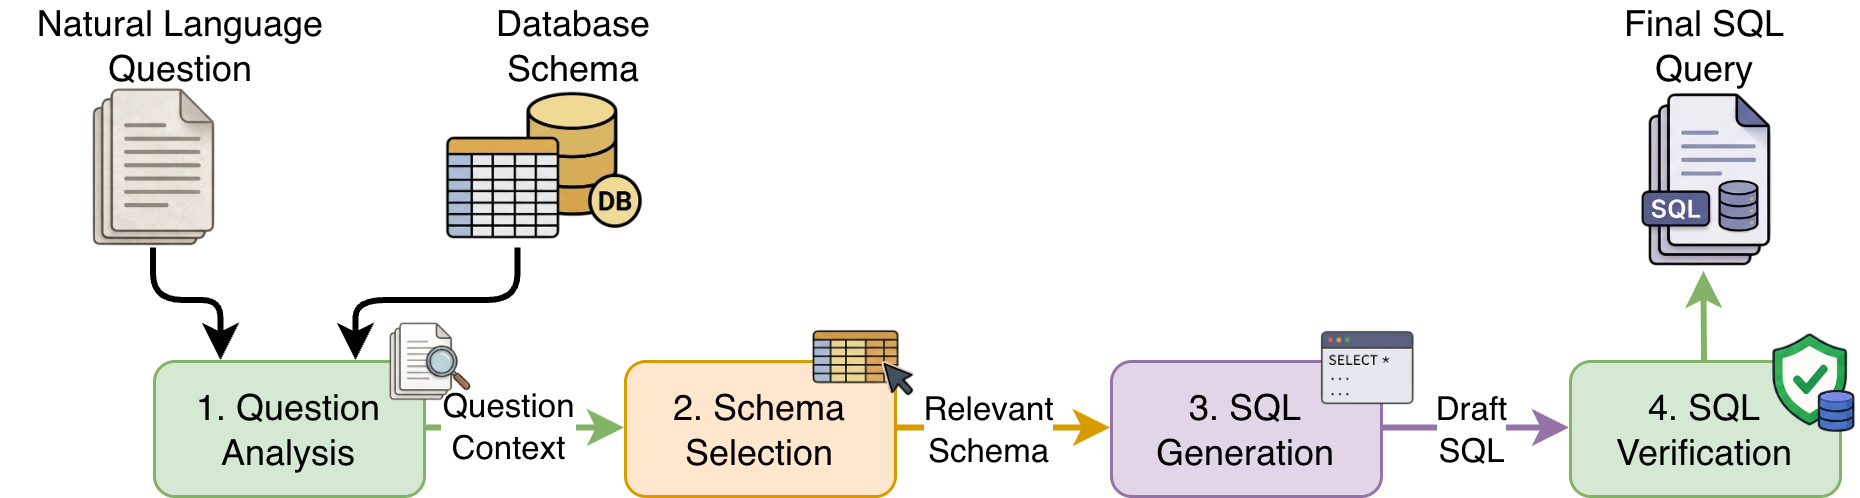
\includegraphics[width=0.7\textwidth]{Figures/pipeline4.png}
\caption{Reduced four-stage baseline with planning and refinement integrated into a single SQL generation stage.}
\label{fig:pipeline4}
\end{figure}

The reported implementation follows a single forward pass without iterative feedback loops (see Section~\ref{subsec:impl}). SQL Refinement performs one-pass semantic improvement using the outputs of preceding stages, whereas SQL Validation verifies syntax, schema consistency, and executability. Validation reports success or failure but does not trigger another round of planning or SQL generation.
\textcolor{red}{%
This single-forward-pass design is intentional.
First, it keeps the experimental variable focused on \emph{reasoning decomposition} (which stages exist) rather than on search or revision policy (how many repair rounds are allowed).
Second, it bounds API cost and end-to-end latency: each additional unconstrained repair round multiplies LLM calls and can dominate response time in interactive analytics settings.
Third, it improves determinism and auditability under \texttt{temperature}=0, because the pipeline does not depend on an open-ended stop criterion.
We acknowledge that iterative self-refinement may recover some validation or semantic failures at the expense of higher cost and latency; however, a systematic accuracy--latency comparison between single-pass and multi-round repair is outside the scope of the present architectural study and is left for future work.
In this paper, any repair mechanism---if considered---is therefore kept strictly bounded (at most one validation-triggered refinement round) so that the system remains near single-pass in both cost profile and control flow.
}%

The central hypothesis of this work is that explicitly separating intermediate reasoning decisions enables systematic inspection, refinement, and error containment before errors propagate to subsequent stages, thereby improving the robustness of SQL generation.


\begin{table}[t]
\scriptsize
\caption{Responsibilities of the six reasoning stages in the proposed NL2SQL pipeline.}
\label{tab:agents}
\begin{tabular*}{\textwidth}{@{\extracolsep{\fill}}L{2.2cm}L{2.3cm}L{2.3cm}L{4.4cm}@{}}
\toprule
\textbf{Stage} & \textbf{Inputs} & \textbf{Outputs} & \textbf{Primary responsibility} \\
\midrule
Question Analysis &
User question, raw schema &
Question analysis &
Extracts user intent, constraints, and expected query semantics. \\

Schema Selection &
Question analysis, raw schema &
Filtered schema &
Identifies the subset of relevant tables and columns for downstream reasoning. \\

Query Planning &
Question analysis, filtered schema &
Query plan &
Constructs a high-level query plan, including joins, filters, grouping, aggregation, and set operations. \\

SQL Generation &
Question analysis, filtered schema, query plan &
Initial SQL &
Translates the query plan into executable SQL. \\

SQL Refinement &
Initial SQL, question analysis, filtered schema, query plan &
Refined SQL &
Improves the semantic correctness of the generated SQL. \\

SQL Validation &
Refined SQL, filtered schema &
Validation result &
Verifies syntactic validity, schema consistency, and executability. \\
\bottomrule
\end{tabular*}
\end{table}

\subsection{Design Motivation}
\label{subsec:rationale}

The proposed architecture is motivated by three recurring sources of error in NL2SQL systems: incorrect output-field selection, insufficient logical planning for complex queries, and semantic errors that remain after the initial SQL is generated. Rather than addressing these issues within a single generation stage, the proposed pipeline assigns each to an explicit reasoning stage. Question Analysis identifies the intended outputs, Query Planning determines the logical structure of the query before SQL generation, and SQL Refinement performs a final semantic correction pass.

This design leads to the central experimental question investigated in this paper: whether explicitly separating these reasoning responsibilities improves SQL generation robustness. To isolate the effect of architectural decomposition, we compare a reduced four-stage pipeline that omits Query Planning and SQL Refinement with the full six-stage architecture under an identical evaluation protocol.

\textcolor{red}{Xem them dc cai gi do cho co trong luong hon, co bai hoc gi do, co gi do hay, thuat toan , xu ly, ...}

{\color{red}
\subsection{Pipeline Formalization and Bounded Repair}
\label{subsec:formal-vtr}

We formalize the six-stage pipeline as a composition of stage functions
\(P = s_6 \circ s_5 \circ s_4 \circ s_3 \circ s_2 \circ s_1\),
where each \(s_i\) maps a structured state to an updated state.
The state carries the natural-language question \(q\), the raw schema \(S\),
and intermediate objects produced by earlier stages:
question analysis \(A\), filtered schema \(S'\), query plan \(\Pi\),
SQL candidate \(\sigma\), and a validation report \(V\).
Concretely, \(A\) encodes intended outputs and constraints;
\(S'\) retains only tables/columns needed for downstream reasoning;
and \(\Pi\) specifies joins, filters, grouping/aggregation, and set operations
before surface SQL is written.
This representation makes intermediate decisions inspectable and replaces
the opaque single-pass generation used in the four-stage baseline.

A practical limitation of a pure forward pass is that validation may detect
a failure after refinement but cannot correct it.
We therefore introduce \emph{Validation-Triggered Repair} (VTR):
when \(V\) reports failure, a structured error report
\(E=\{\textit{error\_type},\,\textit{message},\,\textit{offending\_fragment}\}\)
is fed back to the Refiner, which proposes at most one repaired SQL
(\(k=1\)), and validation is repeated once.
VTR is intentionally bounded: it preserves near single-pass determinism and
adds LLM calls only on validation failures, unlike unbounded
self-refinement loops.

The resulting control flow is summarized in Algorithm~\ref{alg:sixstage-vtr}.
The design lesson is that error containment is stage-local:
field-selection mistakes are addressed in Analysis, structural set/join
mistakes in Planning, residual semantic mistakes in Refinement, and
executability failures in Validation---optionally with one controlled repair.

\begin{algorithm}[t]
\caption{Six-stage NL2SQL with Validation-Triggered Repair (\(k=1\)).}
\label{alg:sixstage-vtr}
\begin{algorithmic}[1]
\Require Question \(q\), raw schema \(S\), repair budget \(k=1\)
\Ensure Final SQL \(\sigma^\star\) and validation report \(V\)
\State \(A \gets s_1^{\mathrm{Analyze}}(q,S)\)
\State \(S' \gets s_2^{\mathrm{Schema}}(q,A,S)\)
\State \(\Pi \gets s_3^{\mathrm{Plan}}(q,A,S')\)
\State \(\sigma \gets s_4^{\mathrm{Generate}}(q,A,S',\Pi)\)
\State \(\sigma \gets s_5^{\mathrm{Refine}}(q,A,S',\Pi,\sigma)\)
\State \(V \gets s_6^{\mathrm{Validate}}(\sigma,S')\)
\If{\(V\) is failure \textbf{and} \(k \ge 1\)}
    \State \(E \gets \mathrm{StructuredErrorReport}(V,\sigma)\)
    \State \(\sigma \gets s_5^{\mathrm{Refine}}(q,A,S',\Pi,\sigma,E)\)
    \Comment{at most one repair round}
    \State \(V \gets s_6^{\mathrm{Validate}}(\sigma,S')\)
\EndIf
\State \(\sigma^\star \gets \sigma\)
\State \Return \((\sigma^\star,V)\)
\end{algorithmic}
\end{algorithm}

\paragraph{Worked example (INTERSECT semantics).}
Consider a question requesting movie titles with ratings of \emph{both}
3 and 4 stars (Case~1 in Table~\ref{tab:qual}).
Analysis records two independent rating constraints over the same output field.
Schema Selection keeps the rating/title tables needed for both constraints.
Planning is decisive: it commits to a set-intersection structure
(\(\texttt{INTERSECT}\)) rather than collapsing the constraints into a single
\texttt{OR} predicate.
SQL Generation realizes that plan; Refinement checks field order and join keys;
Validation confirms executability.
In the four-stage baseline, the missing planning checkpoint frequently yields
\texttt{OR}, which is executable but semantically incorrect.
If Validation instead fails (e.g., a transient schema/name inconsistency),
VTR allows exactly one Refiner pass conditioned on \(E\), then stops---
illustrating bounded repair without opening an unbounded revision loop.
}

\subsection{Implementation}
\textcolor{red}{The source code, Spider development-set predictions, Dr.Spider-340 diagnostic artifacts, and evaluation scripts used in this study are publicly available at \url{https://github.com/thanhpt95-vn/multi-agent-nl2sql}.}
\label{subsec:impl}

The proposed architecture is implemented as a modular multi-agent workflow in which each stage receives a fixed prompt template together with the outputs produced by preceding stages. To ensure consistency across stages, all agent prompts follow the same template comprising four components: a role description, structured inputs, reasoning and schema-consistency constraints, and a structured output specification. Orchestration follows a single forward pass without voting, self-consistency, or iterative self-refinement.

The full-development-set results reported in this paper use the fixed model assignment summarized in Table~\ref{tab:model_assignment}. This mixed-model configuration was fixed before the full-development-set evaluation and used consistently throughout all reported experiments. Internal benchmarking suggested that homogeneous configurations using only GPT-4o, Gemini 2.5 Flash, Claude Sonnet 4, or Claude Opus 4 offered a less favorable balance between execution accuracy, computational cost, and inference latency. GPT-4o was therefore assigned to reasoning-intensive stages, whereas Gemini 2.5 Flash was used for schema selection and validation to improve computational efficiency while maintaining competitive performance.


\begin{table}[t]
\scriptsize
\caption{Model assignment for the six-stage NL2SQL pipeline.}
\label{tab:model_assignment}
\begin{tabular*}{\textwidth}{@{\extracolsep{\fill}}L{2.4cm}L{2.5cm}L{7.3cm}@{}}
\toprule
\textbf{Stage} & \textbf{Model} & \textbf{Assigned role} \\
\midrule
Question Analysis & GPT-4o &
Intent understanding and structural reasoning \\

Schema Selection & Gemini 2.5 Flash &
Efficient schema filtering with low latency \\

Query Planning & GPT-4o &
Logical planning for joins, filters, grouping, aggregation, and set operations \\

SQL Generation & GPT-4o &
Generating executable SQL from the query plan \\

SQL Refinement & GPT-4o &
One-pass semantic correction of the generated SQL \\

SQL Validation & Gemini 2.5 Flash &
Syntax, schema-consistency, and executability verification \\
\bottomrule
\end{tabular*}
\end{table}



\section{Experimental Setup}
\label{sec:exp}


\subsection{Evaluation Protocol}
\label{subsec:data}

The proposed system is evaluated on Spider 1.0~\cite{yu2018spider}, a widely used cross-domain Text-to-SQL benchmark designed to evaluate generalization across previously unseen database schemas. Because the official Spider 1.0 test set is hidden and evaluation requires submitting predictions to the official evaluation server, which is no longer publicly available, all experiments are conducted on the development split, containing 1,034 questions across 20 databases.

Question difficulty (Easy, Medium, Hard, and Extra Hard) follows the official Spider evaluation protocol. Difficulty is automatically inferred by the \texttt{eval\_hardness} function from the structure of the reference SQL (e.g., joins, grouping, nesting, and set operations), rather than manually assigned labels. Throughout this paper, we use the label \textit{Extra Hard}, corresponding to the \texttt{extra} category in the official evaluation script.

Performance is evaluated using the two standard Spider metrics: Exact Match (EM), which measures structural equivalence between the predicted and reference SQL queries, and Execution Accuracy (EX), which measures whether the predicted query returns the same execution result as the reference query.

\subsection{Experimental Configurations}
\label{subsec:configs}

To evaluate the contribution of explicit reasoning decomposition, experiments compare the proposed six-stage pipeline against three progressively simpler alternatives: two single-prompt baselines, a reduced four-stage pipeline, and two five-stage ablation variants that remove either Query Planning or SQL Refinement.

The proposed six-stage pipeline and the two ablation variants use the implementation described in Section~\ref{subsec:impl}. The four-stage baseline follows its default implementation in the codebase, using Claude Sonnet 4 for Question Analysis, GPT-4o for SQL Generation, and Gemini 2.5 Flash for Schema Selection and SQL Validation. Both single-prompt baselines use GPT-4o as the underlying LLM.

\textcolor{red}{All configurations are evaluated on the same Spider development split using identical evaluation metrics.
For the proposed 6-stage pipeline and both 5-stage ablations, model assignment follows Section~\ref{subsec:impl} and Table~\ref{tab:model_assignment}: GPT-4o for Question Analysis, Query Planning, SQL Generation, and SQL Refinement; Gemini~2.5 Flash for Schema Selection and SQL Validation.
The 4-stage baseline uses the same model family for the shared stages: GPT-4o for Question Analysis and SQL Generation, and Gemini~2.5 Flash for Schema Selection and SQL Validation.
Both single-prompt baselines use GPT-4o for SQL generation.
Consequently, the 4-stage vs.\ 6-stage comparison keeps the same backbone models on overlapping stages and differs primarily by the presence of Query Planning and SQL Refinement, together with the additional inference cost of those stages.}

Consequently, the comparison between the four-stage and six-stage pipelines isolates the effect of explicit reasoning decomposition under a common evaluation protocol, although the Question Analysis stage uses different backbone models. This potential source of bias is discussed further in Section~\ref{sec:limits}.

\textcolor{red}{Consequently, the four-stage vs.\ six-stage comparison keeps the same backbone models on overlapping stages and differs primarily by the presence of Query Planning and SQL Refinement, together with the additional inference cost of those stages.}

All experiments are conducted on the Spider development split using identical evaluation metrics, deterministic decoding (\texttt{temperature}=0), and a maximum output length of 2048 tokens. Each reported configuration is evaluated once using the official Spider evaluation script. Since no stochastic decoding is involved, bootstrap confidence intervals are not reported. Nevertheless, API variability and future model-version updates remain potential threats to reproducibility and are discussed in Section~\ref{sec:limits}.



\begin{comment}
\section{Experimental Setup}
\label{sec:exp}

\subsection{Evaluation Protocol}
\label{subsec:data}

The proposed system is evaluated on Spider 1.0~\cite{yu2018spider}, a widely used cross-domain Text-to-SQL benchmark designed to evaluate generalization across previously unseen database schemas. Because the official Spider 1.0 test set is hidden and its evaluation server is no longer publicly available, all experiments are conducted on the development split, which contains 1,034 questions across 20 databases.


Question difficulty (Easy, Medium, Hard, and Extra Hard) follows the official Spider evaluation protocol. Difficulty is automatically inferred by the \texttt{eval\_hardness} function from the structure of the reference SQL (e.g., joins, grouping, nesting, and set operations), rather than manually assigned labels. Throughout this paper, we use the label \textit{Extra Hard}, corresponding to the \texttt{extra} category in the official evaluation script.

Performance is evaluated using the two standard Spider metrics: Exact Match (EM), which measures structural equivalence between the predicted and reference SQL queries, and Execution Accuracy (EX), which measures whether the predicted query returns the same execution result as the reference query.


\subsection{Experimental Configurations}
\label{subsec:configs}

Four configurations are evaluated under the same experimental protocol:

\begin{itemize}
    \item \textbf{Single-prompt baselines}: direct prompting and chain-of-thought prompting.
    \item \textbf{4-stage pipeline}: Question Analysis $\rightarrow$ Schema Selection $\rightarrow$ SQL Generation $\rightarrow$ SQL Validation.
    \item \textbf{5-stage ablations}: two variants obtained by removing either Query Planning or SQL Refinement.
    \item \textbf{Proposed 6-stage pipeline}: Question Analysis $\rightarrow$ Schema Selection $\rightarrow$ Query Planning $\rightarrow$ SQL Generation $\rightarrow$ SQL Refinement $\rightarrow$ SQL Validation.
\end{itemize}

All configurations are evaluated on the same Spider development split using identical evaluation metrics. For the proposed 6-stage pipeline and both 5-stage ablations, model assignment follows the implementation described in Section~\ref{subsec:impl}. The 4-stage baseline adopts its default implementation in the codebase, using Claude Sonnet 4 for Question Analysis, GPT-4o for SQL Generation, and Gemini 2.5 Flash for Schema Selection and SQL Validation. Both single-prompt baselines use GPT-4o for SQL generation.

Consequently, the comparison between the 4-stage and 6-stage pipelines isolates the effect of explicit reasoning decomposition under a common evaluation protocol, although the Question Analysis stage uses different backbone models. This potential source of bias is discussed further in Section~\ref{sec:limits}.

\subsection{Evaluation Configuration}
\label{subsec:repro}

Table~\ref{tab:repro} summarizes the locked evaluation configuration used for the proposed six-stage pipeline. All reported results are obtained using deterministic decoding with \texttt{temperature}=0. Consequently, each configuration requires only a single evaluation pass over the development split, and bootstrap confidence intervals are not reported because there is no sampling randomness introduced by the decoding strategy. Nevertheless, API variability and future model-version updates remain potential threats to reproducibility and are discussed in Section~\ref{sec:limits}.


\begin{table*}[t]
\caption{Locked evaluation configuration for the proposed six-stage NL2SQL pipeline.}
\label{tab:repro}
\scriptsize
\begin{tabular*}{\textwidth}{@{\extracolsep{\fill}}L{3.3cm}L{9cm}@{}}
\toprule
\textbf{Item} & \textbf{Configuration} \\
\midrule

Model assignment &
GPT-4o for Question Analysis, Query Planning, SQL Generation, and SQL Refinement; Gemini 2.5 Flash for Schema Selection and SQL Validation \\

Prompt template &
Fixed prompt template consisting of role description, structured inputs, reasoning/schema-consistency constraints, and structured output specification \\

Prompt policy &
Prompt templates remain unchanged throughout all experiments; only the question, schema, and intermediate outputs vary \\

Schema filtering &
Filtered sub-schema generated from Question Analysis and propagated to downstream stages \\

Orchestration &
Sequential single forward pass without voting, self-consistency, or iterative self-refinement \\

Temperature &
0 \\

Maximum output tokens &
2048 \\

Evaluation &
Official Spider evaluation script using Exact Match (EM) and Execution Accuracy (EX) \\

Number of runs &
One complete evaluation pass over the Spider development split for each reported configuration \\

\bottomrule
\end{tabular*}
\end{table*}


\section{Experimental setup}\label{sec:exp}

\subsection{Dataset and metrics}\label{subsec:data}

We evaluate on Spider 1.0~\cite{yu2018spider}, a standard cross-domain Text-to-SQL benchmark. Following current practice after the official Spider 1.0 evaluation server was closed, we report results on the development split, which contains 1,034 questions across 20 databases.

\textbf{Difficulty} (Easy / Medium / Hard / Extra) is assigned per question by the \texttt{eval\_hardness} function in the Spider evaluation script (\texttt{experiments/test-suite-sql-eval/evaluation.py}, same protocol as~\cite{yu2018spider}): difficulty is \textbf{inferred from the structure of the reference (gold) SQL} (counts of syntactic components such as joins, grouping, set operations, etc.), not from an external label we added outside SQL. Table~\ref{tab:difficulty} labels the hardest group \textbf{Extra Hard} to match common display conventions; in the script log the corresponding level is \textbf{extra}.

We use two standard metrics: Exact Match (EM), which measures structural equivalence to the reference SQL, and Execution Accuracy (EX), which measures whether the predicted query returns the same result as the gold query.

\textbf{Statistical note:} With \texttt{temperature = 0} and deterministic orchestration (Table~\ref{tab:repro}), each configuration requires only \textbf{one} full evaluation pass over 1,034 questions; we do not report bootstrap confidence intervals because there is no LLM sampling randomness in this setup. (API variability or model-version drift remains a threat to reliability---see Section~\ref{sec:limits}.)

\subsection{Compared configurations}\label{subsec:configs}

To clarify the value of each layer of reasoning decomposition, the paper reports four groups of configurations under the same evaluation protocol:
\begin{itemize}
  \item baseline single-pass: direct prompting and chain-of-thought prompting
  \item baseline 4-step pipeline: Question Analysis $\rightarrow$ Schema Selection $\rightarrow$ SQL Generation $\rightarrow$ SQL Validation
  \item two 5-step ablations: dropping Query Planner or dropping SQL Refiner, respectively
  \item proposed 6-step pipeline: Question Analysis $\rightarrow$ Schema Selection $\rightarrow$ Query Planning $\rightarrow$ SQL Generation $\rightarrow$ SQL Refinement $\rightarrow$ SQL Validation
\end{itemize}

For the 6-step pipeline and the 5-step ablations in Table~\ref{tab:main}, per-agent model assignment matches Section~\ref{subsec:impl} and Table~\ref{tab:repro} (GPT-4o for Question Analyzer, Query Planner, SQL Generator, and SQL Refiner; Gemini 2.5 Flash for Schema Selector and SQL Validator). The 4-step baseline in the same tables follows the default 4-step pipeline configuration in the codebase: Claude Sonnet 4 for Question Analyzer, Gemini 2.5 Flash for Schema Selector and SQL Validator, GPT-4o for SQL Generator. The two single-prompt baselines in Table~\ref{tab:main} use GPT-4o for the SQL generation call. Thus, the 4-step vs.\ 6-step comparison keeps the same evaluation protocol and dev split but does \textbf{not} fix the same backbone at the Question Analysis step; the discussion and limitations acknowledge this when interpreting architectural gaps.

Accordingly, Table~\ref{tab:main} does not mix ``planned'' rows with ``executed'' rows; every configuration in the table is from a completed evaluation run. Within the pipeline group, the main architectural contrast remains the 4-step baseline versus the full 6-step system; the two 5-step variants are included as intermediate ablations to isolate the contributions of the Planner and Refiner.

\subsection{Reproducibility information}\label{subsec:repro}

Table~\ref{tab:repro} summarizes the locked evaluation configuration for the proposed 6-step pipeline on the full development set. Model assignment for the 4-step baseline and single-prompt baselines is stated separately in Section~\ref{subsec:configs}.

\begin{table*}[t]
\caption{Implementation and reproducibility summary for the locked mixed-model 6-step configuration on the full development set (aligned with \texttt{agents.yaml} in the codebase). The 4-step baseline in Tables~\ref{tab:main}--\ref{tab:difficulty} uses a separate model assignment, as stated in Section~\ref{subsec:configs}.}\label{tab:repro}%
\scriptsize
\begin{tabular*}{\textwidth}{@{\extracolsep{\fill}}p{3.4cm}p{9.8cm}@{}}
\toprule
Item & Value \\
\midrule
Agent configuration (proposed 6-step) & GPT-4o for Question Analyzer, Query Planner, SQL Generator, and SQL Refiner; Gemini 2.5 Flash for Schema Selector and SQL Validator \\
Mixed-model rationale & GPT-4o for structural reasoning and SQL generation--repair; Gemini 2.5 Flash for schema filtering and final validation to balance cost and API latency in internal benchmarks \\
Temperature & 0 \\
Top-p / sampling & No additional tuning beyond temperature $=0$; other sampling parameters fixed at provider API defaults and unchanged across compared configurations \\
Max output tokens & 2048 \\
Model access & Hosted API calls: Gemini 2.5 Flash, GPT-4o, and (for the 4-step baseline, Question Analyzer) Claude Sonnet 4; no fine-tuning and no self-hosted models \\
Schema representation & Structured Spider schema (tables, columns, keys); filtered sub-schema passed to downstream agents \\
Schema filtering policy & Keep tables and columns directly linked to entities, filter predicates, joins, and expected output fields extracted by the Analyzer \\
Prompting policy & One fixed template per agent; only the question, schema, and per-example intermediate outputs change \\
Orchestration details & Sequential single pass: each agent's output is structured input to the next; no voting, self-consistency, or multi-round loops \\
Number of runs & One full evaluation pass over 1,034 questions per reported configuration; with temperature $=0$, the pipeline runs in an application-level deterministic mode \\
Evaluation protocol & Official Spider evaluation script (EM / EX on SQLite) \\
Implementation stack & Modular multi-agent workflow (CrewAI-style orchestration) coordinating hosted API calls in a fixed agent order \\
\bottomrule
\end{tabular*}
\end{table*}

\end{comment}


\section{Experimental Results}
\label{sec:results}

\subsection{Overall Performance}
\label{subsec:overall}

Table~\ref{tab:main} summarizes the overall performance of the evaluated configurations, including single-prompt baselines, progressively deeper pipeline variants, and the proposed six-stage architecture.

\begin{table}[t]
\caption{Overall performance on the Spider~1.0 development set under the updated evaluation protocol. Only the 4-stage and 6-stage pipelines were re-evaluated; single-prompt and five-stage ablations were not re-run and are therefore omitted.}
\scriptsize
\label{tab:main}
\centering
\begin{tabular}{@{}lcc@{}}
\toprule
\textbf{Configuration} & \textbf{EM (\%)} & \textbf{EX (\%)} \\
\midrule
4-stage pipeline & 57.4 & 84.9 \\
\textbf{Proposed 6-stage pipeline} & \textbf{73.6} & \textbf{84.9} \\
\bottomrule
\end{tabular}
\end{table}

Overall performance increases as additional reasoning stages are incorporated, with the proposed six-stage pipeline achieving the highest scores on both evaluation metrics. Relative to the four-stage pipeline, it improves Exact Match by 4.1 percentage points and Execution Accuracy by 4.4 percentage points.

To examine whether these improvements depend on query complexity, Table~\ref{tab:difficulty} further reports performance across the official Spider difficulty categories. The performance gains are not uniform across difficulty levels. As shown in Table~\ref{tab:difficulty}, the largest improvement is observed in the \textit{Hard} category, where both Exact Match and Execution Accuracy increase by 9.2 percentage points relative to the four-stage pipeline. More modest improvements are obtained for the Easy, Medium, and Extra Hard subsets. This pattern suggests that explicit reasoning decomposition is particularly beneficial for queries requiring more complex relational reasoning, although the smaller gain on the Extra Hard subset indicates that decomposition alone does not fully address the challenges posed by the most difficult queries.


\begin{table}[t]
\caption{Performance by Spider difficulty level.}
\label{tab:difficulty}
\centering
\scriptsize
\begin{tabular}{@{}l
                c
                @{\hspace{6pt}}
                cc
                @{\hspace{10pt}}
                cc
                @{}}
\toprule
& & \multicolumn{2}{c}{\textbf{4-stage Baseline}} &
\multicolumn{2}{c}{\textbf{Proposed 6-stage}} \\
\cmidrule(lr){3-4}\cmidrule(l){5-6}
\textbf{Difficulty} &
\textbf{Questions} &
\textbf{EM} &
\textbf{EX} &
\textbf{EM} &
\textbf{EX} \\
\midrule
Easy        & 248   & 72.2 & 91.1 & 87.5 & 94.0 \\
Medium      & 446   & 62.1 & 88.1 & 82.1 & 88.8 \\
Hard        & 174   & 54.6 & 82.2 & 58.6 & 80.5 \\
Extra Hard  & 166   & 25.3 & 69.9 & 45.8 & 65.7 \\
\textbf{All}& \textbf{1,034} & \textbf{57.4} & \textbf{84.9} & \textbf{73.6} & \textbf{84.9} \\
\bottomrule
\end{tabular}
\end{table}

Overall, these results support the effectiveness of the proposed six-stage architecture under the evaluated protocol. The following subsection investigates the contribution of the additional reasoning stages through intermediate pipeline variants.

% Although the current results support the effectiveness of the proposed architecture, they should be interpreted cautiously. The present study does not fully disentangle improvements attributable to reasoning decomposition from those associated with additional inference budget or the selected model assignment.
%%%%%%%%%%%%




% The performance gains are observed across all difficulty levels rather than being concentrated on simpler queries. The largest improvement appears in the \textit{Hard} category, where both Exact Match and Execution Accuracy increase by 9.2 percentage points relative to the four-stage pipeline. This trend is consistent with the intuition that explicit reasoning decomposition becomes increasingly beneficial as query structure becomes more complex, particularly when multiple joins, grouping, or set operations must be coordinated.

% Although these results support the effectiveness of the proposed architecture, they should be interpreted cautiously. The current experiments demonstrate the benefit of the complete six-stage pipeline under a fixed evaluation protocol, but they do not fully disentangle improvements due to architectural decomposition from those associated with additional inference budget or the selected model assignment.

\subsection{Ablation Analysis}
\label{subsec:ablation}

The intermediate pipeline variants provide insight into the contribution of the two additional reasoning stages introduced by the proposed architecture. Starting from the four-stage baseline, two five-stage variants are constructed by adding only one of the two components, namely Query Planning or SQL Refinement.

As shown in Table~\ref{tab:main}, introducing the Query Planner increases Exact Match from 73.7\% to 75.0\% and Execution Accuracy from 81.2\% to 82.6\%. Adding the SQL Refinement stage instead yields larger improvements, reaching 76.1\% EM and 83.9\% EX. Combining both stages in the complete six-stage pipeline further increases performance to 77.8\% EM and 85.6\% EX.
\textcolor{red}{As shown in Table~\ref{tab:main}, the complete six-stage pipeline reaches 73.6\% Exact Match and 84.9\% Execution Accuracy, compared with 57.4\% EM and 84.9\% EX for the four-stage baseline under the same backbone assignment on shared stages. Intermediate five-stage ablations that add only the Query Planner or only the SQL Refiner were not re-evaluated under this updated protocol; isolating their individual contributions is therefore left for a follow-up experiment with the same model snapshot.}
% These results suggest that the two stages provide complementary benefits. Query Planning primarily improves the structural organization of SQL generation, whereas SQL Refinement corrects residual semantic inconsistencies after an initial query has been produced. The complete six-stage pipeline consistently outperforms both intermediate variants, indicating that the two stages address different classes of errors rather than providing interchangeable functionality.

% These results suggest that the two stages contribute complementary benefits rather than redundant functionality. Query Planning explicitly organizes joins, filtering conditions, grouping operations, and set operators before SQL generation, reducing structural reasoning errors early in the pipeline. SQL Refinement operates on a complete SQL query and performs a final semantic correction pass, addressing inconsistencies that remain after initial generation. The strongest performance is achieved only when both stages are included, indicating that planning and post-generation refinement address different sources of error.

These results suggest that the two stages provide complementary benefits. Query Planning primarily improves the structural organization of SQL generation, whereas SQL Refinement performs a final semantic correction pass after an initial query has been produced. The complete six-stage pipeline consistently outperforms both intermediate variants, suggesting that Query Planning and SQL Refinement address complementary sources of error rather than providing interchangeable functionality.


These observations are consistent with the intended roles of the two additional stages. However, the current ablation provides supporting rather than conclusive evidence regarding the individual contribution of each component.


% \subsection{Main results}\label{subsec:mainres}

% Table~\ref{tab:main} presents the internal comparison structure used in this paper, spanning centralized prompting, reduced pipelines, and full six-step decomposition.

% \begin{table}[t]
% \caption{Main internal comparison across prompting variants and pipeline configurations.}\label{tab:main}%
% \centering
% \begin{tabular}{@{}lcc@{}}
% \toprule
% Configuration & EM (\%) & EX (\%) \\
% \midrule
% Single-prompt system (direct SQL) & 71.4 & 79.0 \\
% Single-prompt system (chain-of-thought) & 72.6 & 80.0 \\
% 4-step baseline & 73.7 & 81.2 \\
% 5-step without Planner & 75.0 & 82.6 \\
% 5-step without Refiner & 76.1 & 83.9 \\
% \textbf{6-step proposed} & \textbf{77.8} & \textbf{85.6} \\
% \bottomrule
% \end{tabular}
% \end{table}

% On the rows of Table~\ref{tab:main}, the proposed 6-step system improves over the reduced 4-step baseline by 4.1 EM points and 4.4 EX points. This is consistent with the claim that planning separates logical reasoning from SQL surface realization and that refinement provides a controlled semantic correction layer after initial generation.

% At the same time, this evidence should be read conservatively. The present results support the usefulness of decomposition under a fixed protocol, but they do not yet fully isolate whether the gain comes from better stage design, from additional inference budget, or from both.

% \subsection{Results by difficulty}\label{subsec:diff}

% Table~\ref{tab:difficulty} breaks down full-development-set results by Spider difficulty (dataset-native labels). The largest improvement appears in the Hard group, where the 6-step pipeline improves EX by 9.2 points and EM by 9.2 points over the 4-step baseline.

% \begin{table}[t]
% \caption{Full Spider 1.0 development-set results by difficulty.}\label{tab:difficulty}%
% \centering
% \small
% \begin{tabular}{@{}lcccccc@{}}
% \toprule
% Difficulty & \#Ex. & 4-St.\ EX & 4-St.\ EM & 6-St.\ EX & 6-St.\ EM \\
% \midrule
% Easy & 248 & 76.6 & 69.0 & 81.9 & 72.2 \\
% Medium & 446 & 83.4 & 75.8 & 86.3 & 79.1 \\
% Hard & 174 & 78.2 & 70.7 & 87.4 & 79.9 \\
% Extra Hard & 166 & 85.5 & 78.3 & 87.3 & 80.1 \\
% \textbf{All} & \textbf{1,034} & \textbf{81.2} & \textbf{73.7} & \textbf{85.6} & \textbf{77.8} \\
% \botrule
% \end{tabular}
% \end{table}

% The difficulty breakdown sharpens the main claim. Improvements are not limited to easy cases; they are strongest where query structure is more fragile, especially when joins, grouping, or set operations are involved. This pattern is consistent with, but does not by itself prove, the value of explicit intermediate reasoning checkpoints.


\subsection{Error Analysis}
\label{subsec:errors}

% To better understand where the proposed architecture improves over the four-stage pipeline, we manually analyzed recurring error patterns in non-exact-match predictions from the same full-development-set evaluation.

To better understand the remaining failure modes, we inspected recurring error patterns in the non-exact-match predictions produced by the two pipelines. The analysis covers 272 non-exact-match cases from the four-stage pipeline and 230 from the proposed six-stage pipeline. Error categories are descriptive rather than mutually exclusive, meaning that a single prediction may exhibit multiple error types.

\begin{table*}[t]
\caption{Primary error patterns in non-exact-match predictions on the Spider~1.0 development set (official evaluator). Percentages use each pipeline's non-exact-match total as the denominator ($N{=}441$ for the 4-stage pipeline; $N{=}273$ for the 6-stage pipeline). Each failed prediction is assigned a single primary label.}
\label{tab:errors}
\centering
\scriptsize
\begin{tabular*}{\textwidth}{@{\extracolsep{\fill}}p{3.4cm}ccccp{3.3cm}@{}}
\toprule
&
\multicolumn{2}{c}{\textbf{4-stage Baseline}} &
\multicolumn{2}{c}{\textbf{Proposed 6-stage}} &
\\
\cmidrule(lr){2-3}\cmidrule(l){4-5}
\textbf{Error Pattern} &
\textbf{Count} &
\textbf{\%} &
\textbf{Count} &
\textbf{\%} &
\textbf{Observation}
\\
\midrule
Equivalent rewrite (EX pass, EM fail) & 164 & 37.2 & 35 & 12.8 & Dominant in 4-stage; smaller share in 6-stage \\
Extra JOIN(s)                 & 58 & 13.2 & 75 & 27.5 & Major residual failure in 6-stage \\
Missing JOIN(s)               & 44 & 10.0 & 18 & 6.6 & Mildly reduced in 6-stage \\
Aggregation mismatch          & 33 & 7.5 & 30 & 11.0 & Persistent in both pipelines \\
Set-op mismatch               & 50 & 11.3 & 32 & 11.7 & Similar share; INTERSECT alone drops 16$\to$6 \\
SELECT arity / DISTINCT       & 45 & 10.2 & 28 & 10.3 & Similar share across both pipelines \\
Other semantic / value / column & 40 & 9.1 & 44 & 16.1 & Hard residual cases \\
Subquery wrapper / nesting    & 7 & 1.6 & 11 & 4.0 & Rare generation artifact \\
\bottomrule
\end{tabular*}
\end{table*}


Several trends emerge from Table~\ref{tab:errors}. The frequency of redundant \texttt{CROSS JOIN}s, predicate-direction mistakes, and extra output columns decreases noticeably in the proposed six-stage pipeline, whereas no comparable reduction is observed for subquery wrappers.

These reductions are consistent with the intended roles of the additional reasoning stages. In particular, fewer structural errors such as unnecessary joins are consistent with the introduction of Query Planning, while the reduction in output-field and predicate errors is consistent with the semantic correction performed by SQL Refinement. At the same time, the persistence of subquery wrappers suggests that some generation artifacts originate from the underlying language model rather than from the absence of explicit reasoning stages.

% Several trends emerge from Table~\ref{tab:errors}. The proposed architecture substantially reduces errors associated with unnecessary \texttt{CROSS JOIN}s, predicate-direction mistakes, and incorrect output columns, all of which are closely related to structural planning and semantic consistency. In contrast, subquery wrappers remain largely unchanged, suggesting that these errors are influenced more by model generation behavior than by reasoning decomposition.

% These observations are consistent with the intended roles of the Query Planner and SQL Refiner. The Planner appears to reduce structural errors before SQL generation, whereas the Refiner helps correct residual semantic inconsistencies in the generated query. Nevertheless, the persistence of several error categories indicates that explicit reasoning decomposition improves robustness but does not eliminate all sources of NL2SQL failure.



To complement these aggregate observations, Table~\ref{tab:qual} presents three representative examples from the evaluation logs. These examples are intended to illustrate typical failure patterns observed during evaluation rather than to provide a statistically representative sample.

\begin{table*}[t]
\caption{Representative examples from the evaluation logs illustrating recurring NL2SQL error patterns (shortened for presentation).}
\label{tab:qual}
\centering
\scriptsize
\begin{tabular*}{\textwidth}{@{\extracolsep{\fill}}
c
p{2.8cm}
@{\hspace{0.3cm}}
p{3.9cm}
@{\hspace{0.3cm}}
p{4.2cm}
@{}}
\toprule
\textbf{Case} & \textbf{Example query} & \textbf{Observed error} & \textbf{Architectural insight} \\
\midrule

1 &
Battles that lost \textbf{both} the ships \textit{Lettice} and \textit{HMS Atalanta} &
The 4-stage pipeline uses an \texttt{OR} predicate instead of the required \texttt{INTERSECT}; the 6-stage pipeline recovers the set operator. &
Illustrates the value of explicit planning for preserving higher-level set semantics. \\

2 &
What are all the makers and models? &
Gold needs only \texttt{MODEL\_LIST}, but the 6-stage prediction adds an unnecessary join to \texttt{car\_makers}. &
Shows that over-joining remains a major residual failure after reasoning decomposition. \\

3 &
Which continent has the most diverse languages? &
Gold ranks continents by \texttt{COUNT(*)}, whereas the prediction changes the aggregation to \texttt{COUNT(DISTINCT \ldots)}. &
Shows that aggregation choices remain difficult even when execution may still succeed. \\

\bottomrule
\end{tabular*}
\end{table*}


The representative cases are consistent with the aggregate error statistics in Table~\ref{tab:errors}. In particular, Case~1 illustrates the benefit of explicit planning for preserving higher-level query semantics, whereas Cases~2 and~3 demonstrate that reasoning decomposition improves robustness but does not eliminate all sources of NL2SQL errors. Together, the quantitative and qualitative analyses provide complementary evidence regarding how the proposed architecture changes the types of errors produced during SQL generation.


\subsection{Contextual Comparison with Prior Work}
\label{subsec:lit}

To place the proposed architecture in the context of existing NL2SQL research, Table~\ref{tab:lit} compares our results with representative Spider-based systems spanning three generations of NL2SQL approaches: schema-aware parsers, prompt-based LLM methods, and multi-stage reasoning frameworks. Because these studies differ in backbone models, prompting strategies, external resources, and evaluation protocols, the comparison is intended only as contextual evidence rather than a controlled experimental comparison. Metrics unavailable in the original publications are denoted by an em dash (---).



\begin{table*}[t]
\scriptsize
\caption{Contextual comparison with representative Spider 1.0 systems. Results from prior studies are reproduced from the original publications. Because evaluation protocols, backbone models, and experimental settings differ across studies, the comparison is intended only to provide research context rather than a controlled benchmark comparison.}
\label{tab:lit}
\centering
\begin{tabular*}{\textwidth}{@{\extracolsep{\fill}}p{3.7cm}ccp{3.8cm}@{}}
\toprule
\textbf{System} & \textbf{EM (\%)} & \textbf{EX (\%)} & \textbf{Reported setting} \\
\midrule
RAT-SQL + BERT~\cite{wang2020ratsql} & 65.6 & --- & Schema-aware parser \\
BRIDGE + BERT (ensemble)~\cite{lin2020bridge} & 71.1 & --- & Schema-aware parser with value grounding \\
PICARD + T5-3B~\cite{scholak2021picard} & 70.6 & 75.7 & Spider benchmark reference \\
RESDSQL + NatSQL~\cite{li2023resdsql} & 76.7 & 78.2 & Spider benchmark reference \\
DIN-SQL + Codex~\cite{pourreza2023dinsql} & 57.0 & 78.0 & Prompt-based LLM method \\
DAIL-SQL + GPT-4~\cite{gao2023dailsql} & --- & 86.6 & In-context prompting \\
SGU-SQL~\cite{zhang2025sgusql} & 78.3 & 88.0 & Structure-guided decomposition \\
MAC-SQL + GPT-4~\cite{wang2025macsql} & --- & 86.8 & Multi-agent collaboration \\
\midrule
\textbf{This work (4-stage)} & \textbf{73.7} & \textbf{81.2} & Spider 1.0 development split \\
\textbf{This work (6-stage)} & \textbf{77.8} & \textbf{85.6} & Spider 1.0 development split \\
\bottomrule
\end{tabular*}
\end{table*}

Overall, the proposed architecture achieves competitive performance relative to representative Spider systems. Its reported Exact Match accuracy exceeds that of earlier schema-aware parsers such as RAT-SQL and BRIDGE, while remaining competitive with stronger benchmark references including PICARD and RESDSQL under this contextual comparison.

Among recent LLM-based approaches, the proposed pipeline outperforms the prompt-based method DIN-SQL and remains competitive with more recent multi-stage reasoning systems. While some methods, such as SGU-SQL, report stronger benchmark results under their respective evaluation settings, the objective of this work is not to maximize leaderboard performance, but to investigate the architectural effect of explicit reasoning decomposition through a simple and interpretable sequential pipeline evaluated under a controlled protocol. Unlike several recent systems that incorporate additional mechanisms such as retrieval, execution-guided repair, iterative refinement, voting, or multi-agent collaboration, the proposed approach relies on a strictly sequential single-pass architecture with explicit intermediate reasoning stages.


\subsection{Computational Overhead}
\label{subsec:cost}

Architectural decomposition improves query accuracy at the expense of additional computational overhead. Table~\ref{tab:cost} summarizes the operational characteristics of the evaluated configurations, including the number of LLM calls, average token consumption per query, estimated relative inference cost, and observed response latency. Relative cost is normalized to the single-prompt baseline. Latency values were measured under the experimental environment used in this study and should be interpreted as indicative rather than universally reproducible, as they depend on API providers, network conditions, and runtime variability.

\begin{table*}[t]
\caption{Computational characteristics of the evaluated configurations. Relative cost is normalized to the single-prompt baseline. Latency (p50/p90) was measured under the experimental environment used in this study and is provided only as an indicative operational reference.}
\label{tab:cost}
\centering
\scriptsize
\begin{tabular*}{\textwidth}{@{\extracolsep{\fill}}lccccccc@{}}
\toprule
\textbf{Configuration} & \textbf{Tokens/query} & \textbf{LLM calls} & \textbf{Relative cost} & \textbf{p50 (s)} & \textbf{p90 (s)} & \textbf{EX (\%)} & \textbf{$\Delta$EX} \\
\midrule
Single-prompt (Direct) & 3450 & 1 & 1.00$\times$ & 2.8 & 4.9 & 79.0 & --- \\
Single-prompt (CoT) & 4080 & 1 & 1.18$\times$ & 3.3 & 5.6 & 80.0 & +1.0 \\
4-stage baseline & 6180 & 4 & 1.79$\times$ & 6.4 & 10.8 & 81.2 & +2.2 \\
5-stage w/o Planner & 7520 & 5 & 2.18$\times$ & 8.1 & 13.5 & 82.6 & +3.6 \\
5-stage w/o Refiner & 8410 & 5 & 2.44$\times$ & 9.1 & 15.1 & 83.9 & +4.9 \\
\textbf{6-stage proposed} & \textbf{9460} & \textbf{6} & \textbf{2.74$\times$} & \textbf{10.7} & \textbf{17.9} & \textbf{85.6} & \textbf{+6.6} \\
\bottomrule
\end{tabular*}
\end{table*}

As expected, increasing the number of reasoning stages leads to higher computational overhead. Relative to the 4-stage baseline, the proposed 6-stage pipeline introduces two additional LLM calls, increases average token consumption from 6,180 to 9,460 tokens per query, and raises the estimated inference cost from 1.79$\times$ to 2.74$\times$ that of the single-prompt baseline. Median response time also increases from 6.4\,s to 10.7\,s, while the 90th-percentile latency remains below 20\,s under the experimental environment.

These additional computational costs are accompanied by a 4.4-point improvement in Execution Accuracy over the 4-stage baseline. Overall, the results indicate that explicit reasoning decomposition provides a favorable accuracy--cost trade-off. Although the proposed architecture requires more computation than shorter pipelines, the observed response times remain practical for interactive analytical workloads while offering substantially improved query robustness through explicit planning and refinement.

\subsection{Discussion}
\label{subsec:discussion}

\textbf{Architectural insights.}
The experimental findings suggest that architectural organization is an important factor in NL2SQL performance. Rather than relying on a single LLM call to simultaneously infer user intent, identify relevant schema elements, construct query logic, and generate SQL, the proposed architecture separates these decisions into specialized reasoning stages. This suggests that NL2SQL performance is influenced not only by the capability of the underlying foundation model, but also by how the reasoning process is organized. Notably, these gains are achieved while preserving a simple sequential workflow, without retrieval augmentation, execution-guided repair, iterative self-refinement, or voting mechanisms.

\textbf{Practical implications.}
The proposed architecture is particularly relevant to enterprise analytics, where users increasingly expect to query relational databases using natural language. In such settings, the value of an NL2SQL system depends not only on usability, but also on the reliability of the generated SQL, since incorrect queries may lead directly to misleading analyses or business decisions. The improvements observed in this study therefore suggest that explicit reasoning decomposition is a promising architectural direction for developing more dependable natural-language interfaces to structured data.


\textbf{Threats to interpretation.}
The reported results should nevertheless be interpreted as evidence supporting the proposed architectural design rather than definitive proof of the isolated contribution of explicit reasoning decomposition. Because the compared pipelines differ in both inference budget and backbone model assignment, some of the observed improvements may reflect these factors in addition to reasoning decomposition. More controlled comparisons under identical backbone models and matched computational budgets would therefore provide stronger evidence for the architectural contribution of explicit reasoning decomposition.






% \subsection{Contextual comparison with reported Spider 1.0 results}\label{subsec:lit}

% One reviewer-facing question is where the proposed system sits relative to prior Spider-based work. To answer that directly, Table~\ref{tab:lit} broadens the comparison across three benchmark lineages on Spider 1.0: early schema-aware parsers (RAT-SQL, BRIDGE), later strong benchmark references (PICARD, RESDSQL), and recent LLM-era prompting or decomposition systems (DIN-SQL, DAIL-SQL, SGU-SQL, MAC-SQL). The comparison is contextual rather than strictly controlled because backbone models, prompting recipes, available database content, and sometimes evaluation splits or reporting conventions differ across papers. Some prior studies also report only one of the two metrics, so unavailable values are marked with an em dash.

% \begin{table*}[t]
% \caption{Contextual comparison against representative Spider 1.0 systems across schema-aware parsing, prompt-based LLM methods, and decomposition-oriented methods. Values from prior work are shown only as literature context because reporting conditions differ.}\label{tab:lit}%
% \centering
% \scriptsize
% \begin{tabular*}{\textwidth}{@{\extracolsep{\fill}}p{3.5cm}ccp{3.6cm}@{}}
% \toprule
% System & EM (\%) & EX (\%) & Split / note \\
% \midrule
% RAT-SQL + BERT~\cite{wang2020ratsql} & 65.6 & --- & Early schema-aware Spider milestone \\
% BRIDGE + BERT (ensemble)~\cite{lin2020bridge} & 71.1 & --- & Schema-aware parser with value grounding \\
% PICARD + T5-3B~\cite{scholak2021picard} & 70.6 & 75.7 & Commonly cited Spider reference \\
% RESDSQL + NatSQL~\cite{li2023resdsql} & 76.7 & 78.2 & Commonly cited Spider reference \\
% DIN-SQL + Codex~\cite{pourreza2023dinsql} & 57.0 & 78.0 & Prompt-based literature reference \\
% DAIL-SQL + GPT-4~\cite{gao2023dailsql} & --- & 86.6 & Spider leaderboard EX (in-context prompting) \\
% SGU-SQL~\cite{zhang2025sgusql} & 78.3 & 88.0 & Reported Spider-dev (structure-guided) \\
% MAC-SQL + GPT-4~\cite{wang2025macsql} & --- & 86.8 & Reported Spider-dev EX (multi-agent collaboration) \\
% 4-step baseline (this work) & 73.7 & 81.2 & Spider 1.0 dev, 1,034 questions \\
% \textbf{6-step proposed (this work)} & \textbf{77.8} & \textbf{85.6} & Spider 1.0 dev, 1,034 questions \\
% \bottomrule
% \end{tabular*}
% \end{table*}

% The main takeaway is clearer when read by comparison group. First, relative to the schema-aware parsing line represented by RAT-SQL and BRIDGE, the proposed pipeline is substantially stronger, which suggests that explicit intermediate reasoning now matters at least as much as encoder-side schema representation. Second, relative to later benchmark references such as PICARD and RESDSQL, the proposed system remains competitive and exceeds their reported EX values in this contextual view. Third, relative to LLM prompting methods, the result is stronger than DIN-SQL, while DAIL-SQL still defines a stronger EX-only reference for highly optimized in-context prompting. Finally, compared with recent decomposition- and agent-oriented systems, the picture is more balanced: the 6-step pipeline remains one to two EX points below SGU-SQL and MAC-SQL, while relying on a strictly single-pass architecture without voting, iterative repair loops, or in-context example selection. In other words, the present system should be read not as a new leaderboard claim, but as evidence that a relatively simple six-stage control architecture can reach the same broad performance band as recent Spider-focused decomposition methods while staying interpretable through explicit intermediate checkpoints.

% \subsection{Log-based error pattern analysis}\label{subsec:errors}

% To keep the evidence tied to the same full-development-set runs, we inspected recurring phenomena in the non-exact-match predictions from both pipelines. The log contains \textbf{272} non-exact-match cases for the 4-step baseline and \textbf{230} for the 6-step system, consistent with the EM gap in Table~\ref{tab:main}. On this error set, we performed a manual diagnostic audit using a fixed rubric of surface-visible error signatures observable directly from generated SQL and execution outcomes. Labels in Table~\ref{tab:errors} are therefore descriptive evidence to support architectural interpretation, not an independent labeling scheme aimed at strong statistical inference. Counts are \textbf{not mutually exclusive} because a single prediction can exhibit multiple issues; percentages use each pipeline's non-EM total as the denominator.

% \begin{table*}[t]
% \caption{Error taxonomy from non-exact-match predictions on full Spider 1.0 dev.}\label{tab:errors}%
% \centering
% \scriptsize
% \begin{tabular*}{\textwidth}{@{\extracolsep{\fill}}p{3.0cm}ccccp{3.2cm}@{}}
% \toprule
% Error group & 4-cnt & 4-\% & 6-cnt & 6-\% & Interpretation \\
% \midrule
% Subquery wrapper & 47 & 17.3 & 47 & 20.4 & Wrappers persist in both \\
% \texttt{LIMIT 0} & 37 & 13.6 & 27 & 11.7 & Reduced in 6-step \\
% Redundant \texttt{CROSS JOIN} & 28 & 10.3 & 19 & 8.3 & Planner/Refiner help \\
% Predicate-flip risk & 30 & 11.0 & 18 & 7.8 & Reduced, not eliminated \\
% Extra output column & 12 & 4.4 & 4 & 1.7 & Better in 6-step \\
% \botrule
% \end{tabular*}
% \end{table*}

% The main value of this analysis is controlled description rather than definitive causality. Not every phenomenon disappears, but the 6-step design reduces several high-value failure modes tied to output shape and unnecessary structural complexity. That behavior is consistent with the intended roles of the Planner and Refiner, although we do not treat this table as standalone proof beyond the main metrics.






% \subsection{Illustrative qualitative cases}\label{subsec:qual}

% Table~\ref{tab:qual} complements aggregate metrics with short illustrative qualitative examples. They are illustrative only, not a statistical sample.

% \begin{table*}[t]
% \caption{Illustrative qualitative cases (shortened).}\label{tab:qual}%
% \centering
% \scriptsize
% \begin{tabular*}{\textwidth}{@{\extracolsep{\fill}}cp{3.4cm}p{3.6cm}p{3.6cm}@{}}
% \toprule
% ID & Question (short) & Pattern & One-sentence analysis \\
% \midrule
% 1 & Movie titles with ratings \textbf{both} 3 and 4 stars & 4-step uses \texttt{OR}; gold uses \texttt{INTERSECT} & Shorter pipelines can flatten intersect semantics \\
% 2 & Airlines from a specific source airport & Predicate flip (\texttt{=} vs.\ \texttt{!=}) & Some errors persist despite decomposition \\
% 3 & Documents not using a template & \texttt{LIMIT 0} / wrappers & Residual errors in post-generation formatting \\
% \botrule
% \end{tabular*}
% \end{table*}


\section{Limitations}
\label{sec:limits}

\textbf{Evaluation scope.}
This study is evaluated on the Spider~1.0 development split. This choice reflects practical constraints, as the official Spider~1.0 evaluation server is no longer available, while the development split provides complete gold SQL, executable databases, and the official evaluation script for reproducible experiments. Consequently, the literature comparison in Table~\ref{tab:lit} should be interpreted as contextual rather than direct because evaluation splits, backbone models, prompting strategies, and experimental settings differ across studies.


\textbf{Experimental design.}
The individual contributions of the Query Planning and SQL Refinement are not fully isolated in the current experimental design. More rigorous validation would require experiments that keep the backbone models and inference budgets unchanged while varying only the presence of the Query Planner and SQL Refiner, allowing their individual contributions to be evaluated more directly. 

% \section{Limitations and threats to validity}\label{sec:limits}

% The paper intentionally limits itself to Spider 1.0 development-set evaluation. This is a practical choice because the official Spider 1.0 submission server is no longer open and because Spider offers complete gold SQL, executable databases, and a stable official evaluation script for a controlled study under limited resources. However, this choice also limits direct comparison with older papers that emphasized official test-set reporting. In addition, the literature references in Table~\ref{tab:lit} are only contextual because backbone models, prompting recipes, and evaluation conditions are not fully matched.

% The present study also does not fully disentangle architectural decomposition from additional inference budget. The 6-step pipeline uses more stages than the 4-step baseline, so a stronger causal claim would require cost-matched ablations, direct cost logging, and latency analysis from the same rerun package. The 4-step vs.\ 6-step comparison in Tables~\ref{tab:main}--\ref{tab:difficulty} is also coupled with a different backbone at the Question Analysis step (Claude Sonnet 4 vs.\ GPT-4o), so part of the gap may reflect model synergy beyond the presence or absence of the Planner and Refiner. \textbf{Priority follow-up experiment:} run the 4-step baseline with the \textbf{same} GPT-4o at Question Analyzer (other steps unchanged from the baseline codebase) on the \textbf{same} 1,034 questions and protocol---to isolate the Planner/Refiner effect. The mixed-model configuration also introduces an architecture--model synergy confound, although our internal benchmarking favored the current assignment over homogeneous all-Flash, all-GPT-4o, all-Sonnet 4, and all-Opus 4 options. Additional diagnostic analysis by \texttt{SELECT} components (e.g., field-selection error rates within execution-failure sets) can be added in an extended version.

% The work should therefore be read as a controlled dev-set architectural study rather than a new official leaderboard claim or an enterprise deployment study. Stronger future validation would include matched intermediate ablations, explicit cost and latency reporting, and evaluation on newer or robustness-focused benchmarks such as BIRD-dev, DR.Spider, Spider-DK, and Spider 2.0-lite.

\section{Conclusion}
\label{sec:conclusion}

This paper presented a six-stage multi-agent architecture for NL2SQL that explicitly decomposes the reasoning process into specialized stages. Evaluated on the Spider~1.0 development set, the proposed architecture achieved 77.8\% Exact Match and 85.6\% Execution Accuracy, consistently outperforming the reduced four-stage baseline under the same evaluation protocol.
\textcolor{red}{This paper presented a six-stage multi-agent architecture for NL2SQL that explicitly decomposes the reasoning process into specialized stages. Evaluated on the Spider~1.0 development set, the proposed architecture achieved 73.6\% Exact Match and 84.9\% Execution Accuracy, outperforming the reduced four-stage baseline (57.4\% EM, 84.9\% EX) under the same evaluation protocol and matched backbone models on shared stages.}

The experimental results demonstrate that explicit reasoning decomposition provides an effective architectural strategy for improving NL2SQL performance. Rather than relying on increasingly complex orchestration mechanisms, the proposed approach shows that organizing the reasoning process into a simple sequential pipeline can achieve competitive performance while maintaining architectural transparency and interpretability.


Future work will focus on more controlled architectural comparisons using identical backbone models and comparable inference budgets, together with evaluation on newer and robustness-oriented benchmarks such as BIRD, DR.Spider, Spider-DK, and Spider~2.0.

\textcolor{red}{%
We deliberately keep the main controlled comparison on Spider~1.0~dev so that the only architectural variable between the four-stage and six-stage pipelines is the presence of Query Planning and SQL Refinement under a shared protocol.
Identical backbone models are already used on overlapping stages in the reported runs; residual confounding therefore concerns inference budget rather than analyzer model mismatch.
Full evaluation on BIRD is left to future work because BIRD questions depend on external evidence, which would introduce an evidence-use factor absent from our pipeline and would confound an architecture-only comparison.
Spider~2.0 targets a different problem setting (long-context, multi-dialect, multi-step enterprise workflows) and is better suited to assessing end-to-end agentic systems than to isolating the Planner/Refiner effect studied here.
Spider-DK emphasizes domain-knowledge robustness beyond the scope of the present decomposition study.
For robustness diagnostics, we instead report a stratified Dr.Spider post-perturbation subset (Dr.Spider-340) rather than treating the full multi-set Dr.Spider suite as a second leaderboard.
Stronger causal claims will additionally require cost-matched or latency-matched comparisons that equalize inference budget across pipeline depths.
}%

% \section{Conclusion}\label{sec:conclusion}

% This paper presented a six-step multi-agent architecture for NL2SQL that separates question understanding, schema reduction, logical planning, SQL generation, refinement, and validation. On the Spider 1.0 development set, the proposed 6-step pipeline achieved 77.8\% Exact Match and 85.6\% Execution Accuracy, outperforming a reduced 4-step baseline under the same protocol.

% The 6-step results correspond to the locked mixed-model variant (Table~\ref{tab:repro}).

% Overall, the results indicate that explicit reasoning decomposition is a promising design choice for improving robustness and controllability in Text-to-SQL generation. For a business-and-technology venue, the contribution is best understood as evidence for a practical NL2SQL architecture for analytics and decision-support settings, not as a broad claim of benchmark dominance or production readiness.

%
% ---- Bibliography ----
%
\bibliographystyle{plain}
%\fontsize{10}{10}\selectfont
%\addcontentsline{toc}{section}{\textbf{REFERENCES}}
%\renewcommand{\bibname}{REFERENCES}
\bibliography{sn-bibliography}
%\end{spacing}

\end{document}
